\documentclass[11pt,a4paper]{article}

\usepackage{../notes}

\title{Probability Theory \& Statistics}

\begin{document}

\maketitle
\newpage

\section{Monte Carlo Simulation}

\subsection{Prerequisites}

\begin{itemize}
\item
Inequalities (Law of Large Numbers \& Central Limit Theorem)
\end{itemize}

\subsection{Introduction}

The solutions to many scientific problems involve intractable
high-dimensional integrals. 
Standard deterministic numerical integration
deteriorates rapidly with the dimension of the space. 
Monte Carlo methods are stochastic numerical methods that 
can be used to approximate high-dimensional integrals. 
They have a diverse range of applications:
statistical/quantum physics, econometrics, ecology, epidemiology,
finance, signal processing, weather forecasting, machine learning, and
Bayesian statistics.

\subsection{Approximation of Integrals}

\subsubsection{Riemann Sums}
Many scientific problems require numerical computation of
integrals, i.e.,
\begin{align}
I = \int_{\mathbb{X}}^{}{f(x)}dx
\end{align}
where \(f:\mathbb{X} \rightarrow \mathbb{R}\). 
For simple choices of functions \(f\) and functional spaces \(\mathbb{X}\), 
the integral can be computed exactly, 
but in general we require numerical approximations of \(I\).

When \(\mathbb{X} = [0,1]\), 
then we can estimate \(I\) through,
\begin{align}
{\widehat{I}}_{n} = 
\frac{1}{n}\sum_{i = 0}^{n - 1}{f\left( \frac{i + 1/2}{n} \right)},
\end{align}
called the \emph{Riemann sum approximation}. 
This corresponds to an approximation of the area under 
the curve \(y = f(x)\) by the sum of
the areas of the rectangles (see figure \ref{fig:integration}). 

When \(f\) is differentiable and
\(M = \sup_{x \in [ 0,1]}\left| f^{\prime}(x) \right| < \infty\),%
\footnote{%
There exists some finite maximum derivative 
on the interior of the domain \([0,1]\).} 
then the approximation error is \(O\left( n^{- 1} \right)\).

\emph{Proof}. 
The error of the \(k\)-th rectangle, for
\(k \in \{ 0,\ldots,n - 1\}\) is,
\begin{align}
\varepsilon_{k} = 
\left| \int_{k/n}^{(k + 1)/n}{f(x)}dx - \frac{1}{n}f\left( \frac{(k + 1/2)}{n} \right) \right| = 
\left| \int_{k/n}^{(k + 1)/n}{\left( f(x) - f\left( \frac{(k + 1/2)}{n} \right) \right)dx} \right|
\end{align}
where we have used the fact that for all
\(x,y \in [ a,b]\), 
there exists
\(c \in [ a,b]\) such that,
\begin{align}
f(x) - f(y) = (x - y)f^{\prime}(c).
\end{align}
Using the bound \(M\) on \(f^{\prime}\), 
and the inequality
\begin{align}
\left| \int f(x) \right| \leq \int\left| f(x) \right|
\end{align}
we obtain,
\begin{align}
\varepsilon_{k} \leq \int_{\frac{k}{n}}^{\frac{k + 1}{n}}{\left| f(x) - f\left( \frac{(k + 1/2)}{n} \right) \right|dx} \leq M\int_{\frac{k}{n}}^{\frac{k + 1}{n}}{\left| x - \frac{(k + 1/2)}{n} \right|dx} \leq M\frac{1}{2n^{2}}.
\end{align}
Summing the errors over the \(n\) rectangles yield a total error
\(Mn \times \frac{1}{2n^{2}} = O\left( n^{- 1} \right)\).

\begin{figure}[h!]
\centering
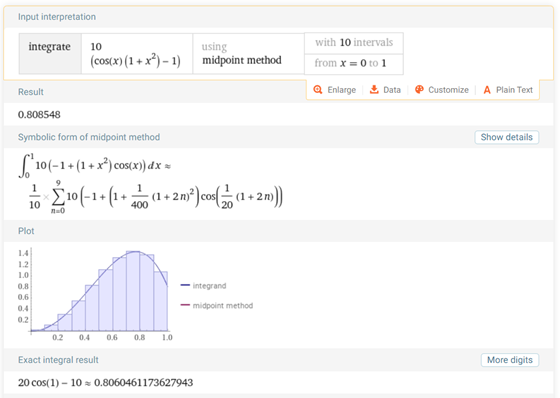
\includegraphics[width=0.75\linewidth]{images/figure1.png}
\caption{%
Numerical integration of %
\(f:x\mapsto 10(\cos(x)\left(1+x^{2}\right)-1)\) from \url{https://www.wolframalpha.com/}.
}
\label{fig:integration}
\end{figure}

\subsubsection{The Curse of Dimensionality}

For \(\mathbb{X}=[0,1] \times [0,1]\)
assuming,
\begin{align}
{\widehat{I}}_{n} = 
\frac{1}{m^{2}}\sum_{i = 0}^{m - 1}{\sum_{j = 0}^{m - 1}{f\left( \frac{i + 1/2}{m},\frac{j + 1/2}{m} \right)}}
\end{align}
and \(n=m^{2}\), 
then the approximation error is \(O\left( n^{- 1/2} \right)\). 
For \(\mathbb{X}=[0,1]^{D}\) therefore, 
the approximation error is in \(O\left(n^{- 1/D} \right)\) 
-- the so-called \emph{curse of dimensionality}. 

This suggests that deterministic approximations
aren't appropriate for computing high-dimensional integrals. 
More sophisticated deterministic approximations like the trapezoidal 
rule or Simpson's rule also suffer 
from the same degeneracy when the dimension increases.

Stochastic simulation methods, 
also known as Monte Carlo methods, 
are the most common tools for performing 
high-dimensional numerical integrations. 
Monte Carlo methods were introduced in the 1940s and have
become extremely popular in statistics 
over the past 20 years because
they make inferences possible in very complex statistical models. 
This session reviews Monte Carlo methods 
and some of their applications in Bayesian statistics and a few other examples.

\subsection{Monte Carlo Integration} % up to here

\subsubsection{Definition}

For \(f:\mathbb{X \rightarrow R}\), write,
\begin{align}
I = \int_{\mathbb{X}}^{}{f(x)}dx = \int_{\mathbb{X}}^{}{\varphi(x)p(x)}dx
\end{align}
where \(p(x)\) is a \emph{probability density function} on \(\mathbb{X}\), and
\begin{align}
\varphi:x \mapsto f(x)/p(x).
\end{align}
A \emph{Monte Carlo method} is defined as:
\begin{itemize}
\item
sample \(X_{1}\), \ldots, \(X_{n} \sim p\),
\item
compute
\begin{align}
{\widehat{I}}_{n} = \frac{1}{n}\sum_{i = 0}^{n}{\varphi(X_{i})}
\end{align}
\end{itemize}
The \emph{strong law of large numbers} guarantees that
\({\widehat{I}}_{n} \rightarrow I\) almost surely, 
and the \emph{central limit theorem} tells us that the random approximation error is,
\begin{align}
O\left(n^{- 1/2}\right)
\end{align}
whatever the dimension of the state space \(\mathbb{X}\)!

\emph{Proof}. 
Non-asymptotically we can prove this result using the mean-square error,
\begin{equation}
\begin{split}
\left( I - {\widehat{I}}_{n} \right)^{2} &= I^{2} - 2I \times {\widehat{I}}_{n} + {\widehat{I}}_{n}^{2} \\
&= I^{2} - \frac{2I}{n}\sum_{i = 0}^{n}{\varphi\left( X_{i} \right)} + \frac{1}{n^{2}}\sum_{i = 0}^{n}{\varphi\left( X_{i} \right)^{2}} + \frac{1}{n^{2}}\sum_{i \neq j}^{n}{\varphi\left( X_{i} \right)\ \varphi(X_{j})}
\end{split}
\end{equation}

As the samples are IID and \(I = E_{p}(\varphi(X))\), we have,
\begin{align}
E_{p}\left( \left( I - {\widehat{I}}_{n} \right)^{2} \right) 
= I^{2} - 2I^{2} + \frac{1}{n}E_{p}\left( \varphi\left( X_{1} \right)^{2} \right) + \frac{1}{n^{2}}n(n - 1)I^{2}\end{align}

\begin{align}= \frac{E_{p}\left( \varphi\left( X_{1} \right)^{2} \right) - I^{2}}{n} = \frac{Var_{p}\left( \varphi\left( X_{1} \right) \right)}{n}\end{align}

Finally,
\(\sqrt{E_{p}\left( \left( I - {\widehat{I}}_{n} \right)^{2} \right)} = \sqrt{\frac{Var_{p}\left( \varphi\left( X_{1} \right) \right)}{n}} \leq \frac{1}{\sqrt{n}}\)
if \(\left| \varphi(x) \right| \leq 1\ \forall x\). Because the r.h.s.
is bounded by a constant, the convergence criterion is independent of
the dimension.

According to the rate \(\sqrt{n}\) of the CLT (Central Limit Theorem),
the variance of the estimator \(I_{n}\) is of order
\(O\left( n^{- 1} \right)\), hence the standard deviation is of order
\(O\left( n^{- 1/2} \right)\). This means that if one wants to divide
the standard deviation by 10 (to obtain ``10 times'' more precision),
one needs to sample 100 times more draws from \(p\), which typically
corresponds to 100 times more computational effort. This rate of
convergence can seem very slow in a single dimension. However, the rate
of convergence does not depend on the dimension \(D_{x}\) of the sample
space \(\mathbb{X}\); it is always \(\sqrt{n}\)!

Thus, Monte Carlo methods converge slower than Riemann sums in one
dimension, whose error was shown to decrease in \(O(n^{- 1})\); they are
of the same accuracy as Riemann sums in two dimensions; and they are
faster than Riemann sums for any dimension \(D_{x} \geq 3\). Thus, Monte
Carlo methods have become standard tools to approximate integrals of
moderate to high dimensions.

In other words, Monte Carlo methods might seem slow, but they are still
typically faster than alternative methods. Bakhvalov, Suldin, and other
mathematicians have proven results on the minimum error that can be
obtained by algorithms using \(n\) pointwise evaluations of \(f\) to
approximate \(\int_{\mathbb{X}}^{}{f(x)}dx\), and the rate
\(n^{- 1/2}\ \)is found to be optimal when the dimension of
\(\mathbb{X}\) is large and/or the ``smoothness'' of \(f\) is low, in
some sense. For instance, the smoothness of \(f\) can be defined as the
maximum integer \(k\) such that all \(k\)-th order partial derivatives
of \(f\) are uniformly bounded on \(\mathbb{X}\).

Note that the rate is \(\sqrt{n}\) uniformly in \(D_{x}\), but
high-dimensional integrals are still harder to approximate than
low-dimensional integrals, as one would expect. Typically, the error
associated with Monte Carlo methods is in \(f(D_{x})/\sqrt{n}\), where
\(f(D_{x})\) is a polynomial in \(D_{x}\), or in the worst case, an
exponential of \(D_{x}\). Thus, the error might still be very large when
\(D_{x}\) is large, as one might not have enough computational power to
scale \(n\) with \(f(D_{x})\). In order to implement the above-described
Monte Carlo method, one needs to obtain IID samples from \(p\). Markov
Chain Monte Carlo methods provide ways to obtain IID samples from
generic distributions \(p\).

In many statistical problems, the integral of interest is an expectation
for the form,

\begin{align}I = \int_{\mathbb{X}}^{}{\varphi(x)\ p(x)}dx = E_{p}\left( \varphi(X) \right),\end{align}

for a specific function \(\varphi\) and density \(p\). The density \(p\)
is then often called the \emph{target density}. The Monte Carlo method
then relies on generating independent copies of,

\begin{align}X \sim p,\end{align}

and replacing the expectations with empirical averages,

\begin{align}E_{p}\left( \varphi(X) \right) \approx \frac{1}{n}\sum_{i = 0}^{n}{\varphi(X_{i})}\end{align}

Hence, the following relationship between integrals and sampling:

Monte Carlo method to approximate \(E_{p}\left( \varphi(X) \right)\) equivalent to
Simulation method to sample \(p\)

The Monte Carlo method is thus often referred to as a simulation method.

\subsection{Applications}\label{applications}

\subsubsection{Volume of a Convex Body}\label{volume-of-a-convex-body}

Let \(S \subset [ 0,\ 1]^{D}\) be a convex body. In numerous
applications, we are interested in computing the volume of this body
given by,

\begin{align}vol(S) = \int_{[ 0,1]^{D}}^{}{\mathbb{I}_{S}(x)}dx\end{align}

where \(\mathbb{I}_{S}(x)\) is the \emph{indicator function}, i.e.,
\(\mathbb{I}_{S}(x) = 1\) if \(x \in S\) and \(0\) otherwise. The
``estimating the value of Pi'' example is in this class of problems --
calculating the volume of a 1-sphere embedded in a \(2D\) space. More
generally, any volume can be approximated by sampling from
\(\mathbb{I}_{S}(X_{i})\) and calculating the empirical average over
\(\mathbb{X}\).

\subsubsection{Statistical Mechanics}\label{statistical-mechanics}

The Ising model is used to model the behaviour of a magnet and is the
best known and most researched model in statistical physics. The
magnetism of a material is modelled by the collective contribution of
dipole moments of many atomic spins.

\begin{figure}[h!]
\centering

\includegraphics[width=0.5\linewidth]{images/figure2.png}
\caption{%
A 2D-Ising model sample.
}
\label{fig:ising}
\end{figure}

Consider a simple \(2D\)-Ising model on a finite lattice
\(\mathcal{G =}\left\{ 1,\ 2,\ \ldots,\ m \right\} \times \{ 1,\ 2,\ ...,\ m\}\)
where each site \(\sigma = (i,\ j)\) hosts a particle with a \(+ 1\) or
\(- 1\) spin, modelled as a random variable \(X_{\sigma}\). The physical
constraints of the system require the probability density of
\(X = \left\{ X_{\sigma} \right\}_{\sigma \in \mathcal{G}}\) on
\(\mathbb{X =}\left\{ - 1,\ 1 \right\}^{m^{2}}\) be given by the Gibbs
distribution,

\begin{align}\forall x \in \mathbb{X,\ \ }p_{\beta}(x) = \frac{\exp\left( - \beta U(x) \right)}{Z_{\beta}}\end{align}

where \(p(x)\) is the \emph{probability density}, \(\beta > 0\) is the
\emph{inverse temperature}, and \(U\) is the \emph{potential energy},

\begin{align}\forall x \in \mathbb{X,\ \ }U(x) = J\sum_{\sigma \sim \sigma^{\prime}}^{}{x_{\sigma}x_{\sigma^{\prime}}},\end{align}

for some \(J\mathbb{\in R}\), where \(\sigma \sim \sigma^{\prime}\) refers to
the set of pairs of sites that are ``neighbours'' in some pre-defined
sense.

For instance, we can define that two sites \(\sigma = (i,\ j)\) and
\(\sigma' = (i^{\prime},\ j^{\prime})\) are neighbors if and only if
\(\left| i - i^{\prime} \right| \leq 1\) and
\(\left| j - j^{\prime} \right| \leq 1\). According to this form of potential
energy, if \(x_{\sigma}\  = \ x_{\sigma^{\prime}}\) and
\(\sigma \sim \sigma^{\prime}\), then the probability \(p_{\beta}(x)\)
includes a term \(\exp{( - J)}\), otherwise it includes a term
\(\exp{(J)}\). Hence the sign of \(J\) tells us whether there is a
preference for equal or opposite spins at sites \(\sigma\) and
\(\sigma^{\prime}\).

The normalizing constant \(Z_{\beta}\) ensures that \(p_{\beta}\) is a
probability distribution, that is,
\(\sum_{x \in \mathbb{X}}^{}{p_{\beta}(x)} = \ 1\). Thus, it is defined
as

\begin{align}Z_{\beta} = \sum_{x \in \mathbb{X}}^{}{\exp\left( - \beta U(x) \right)}.\end{align}

Physicists are often interested in computing \(E_{p_{\beta}}(U(X))\) and
\(Z_{\beta}\). However, analytic results for the Ising model are very
difficult to obtain and physicists often use simulation methods in order
to perform these calculations. Note that the problem of computing sums
is equivalent to the problem of computing integrals and is formally
unified by measure theory.

Although the Ising model was first formulated to solve problems in
statistical mechanics it is a special case of the more general class of
agent-based models and has applications in various fields including
economics and finance.

\subsubsection{Financial Mathematics}\label{financial-mathematics}

Let \(S(t)\) denote the price of a stock at time \(t\). A \emph{call
option} grants the holder the right to buy the stock at a fixed price
\(K\), at a fixed time \(T\) in the future; the current time being
\(t = 0\). The is the so-called \emph{European option}.

If at time \(T\) the stock price \(S(T)\) exceeds the strike price
\(K\), the holder exercises the option for a profit of \(S(T) - K\). If
\(S(T) \leq K\), the option expires worthless. The payoff to the holder
at time \(T\) is thus,

\begin{align}\max\left( S(T) - K \right)^{+} = \max\left( 0,\ S(T) - K \right).\end{align}

The \emph{present value} of the payoff\footnote{Money has an intrinsic
  time-value we need to consider.} is calculated by discounting the
expected future payoff,

\begin{align}V(0) = \exp( - rT)E\left( \max\left( S(T) - K \right)^{+} \right)\end{align}

where \(\exp{( - rT)}\) is the \emph{discount factor}, \(r\) is the
\emph{compounded interest rate}, and \(E\), is an expectation with
respect to the distribution of the random variable \(S(T)\).

If we knew the distribution of \(S(T)\), then computing
\(E\left( \max\left( S(T) - K \right)^{+} \right)\) would be a
low-dimensional integration problem. However, this distribution is
typically not available, and we only have access to a stochastic model
for \(\left\{ S(t) \right\}_{t \in N}\) of the form,

\begin{align}S(t + 1) = g\left( S(t),\ W(t + 1) \right) = g\left( g\left( S(t - 1),\ W(t) \right),\ W(t + 1) \right) = g^{2}\left( S(t - 1),\ W(t),\ W(t + 1) \right) = g^{n}\left( S(0),\ W(1),\ \ldots,\ W(t + 1) \right)\end{align}

where \(W(t)\) is an IID sequence of random variables with probability
density functions \(\left\{ p_{W} \right\}_{t\mathbb{\in N}}\) and \(g\)
is a known nonlinear mapping -- the \emph{payoff function}.

We can rewrite the expectation in the present value equation as

\begin{align}E\left( \max\left( S(T) - K \right)^{+} \right) = \int_{}^{}{{\max\left( g^{n}\left( s(0),\ w(1),\ \ldots,w(T) \right) - K \right)}^{+} \cdot \prod_{t = 1}^{T}{p_{W}\left( w(t) \right)}}\ dw(1)\ldots dw(T)\end{align}

which is a high-dimensional integral whenever \(T\) is large.

\subsection{Bayesian Statistics}\label{bayesian-statistics}

We will now consider several examples from Bayesian statistics. In
statistics the \emph{data} is usually a collection of \(n\) values
\(\left( y_{1},...\ ,\ y_{n} \right) \in \mathcal{Y}^{n}\) in some space
\(\mathcal{Y}\), typically \(\mathbb{R}^{D_{y}}\) for some \(D_{y}\). A
statistical model considers the data to be realisations of random
variables \((Y_{1},\ .\ .\ .\ ,\ Y_{n})\) defined on the same space.
Denote \(Y_{1},\ .\ .\ .\ ,\ Y_{n}\) by \(Y\), and
\(y_{1},\ .\ .\ .\ ,\ y_{n}\) by \(y\). The distribution of these random
variables, which is specified by the model, has a probability density,
\(p_{Y}(y;\theta)\), where \(\theta\) is the parameter of the model
living in some space \(\Theta\).\footnote{Written with respect to some
  dominating measure. This is often required when defining conditional
  probabilities, here the posterior probability.}

The density of the observations, seen as a function of the parameter, is
called the \emph{likelihood}, and is denoted by \(\mathcal{L}_{n}\):

\begin{align}\mathcal{L}_{n}\ :\ \theta \in \Theta \mapsto p_{Y}(y;\theta).\end{align}

In the frequentist approach, \(\theta\) is an unknown fixed value and
inference is performed based on the likelihood function. The standard
estimator is the maximum likelihood estimator
\({\widehat{\theta}}_{n}\), that is the parameter \(\theta\) maximizing
\(\mathcal{L}_{n}(\theta)\) for the dataset
\(\left( y_{1},...\ ,\ y_{n} \right)\). Note, because \(\theta\) is not
random, we write a semi-colon ``;'' in \(p_{Y}(y;\theta)\) instead of a
vertical bar ``\textbar'' to emphasize that this is not a conditional
distribution.

On the contrary, in the Bayesian approach, the unknown parameter is
regarded as the random variable \(\vartheta\), and we assign a prior
probability distribution to it, of density
\(p_{\vartheta}(\theta)\).\footnote{Written with respect to a dominating
  measure denoted \(d\theta\), say a Lebesgue measure if
  \(\Theta = \mathbb{R}^{D_{\theta}}\) for some \(D_{\theta}\))} The
distribution of \(Y\) given \(\vartheta = \theta\) can now be
interpreted as a conditional distribution and we thus denote it by
\(p_{Y|\vartheta}(y\ |\ \theta)\).

Bayesian inference relies on the posterior density,

\begin{align}p_{\vartheta|Y}(\theta\ |\ y) = \frac{p_{Y|\vartheta}(y\ |\ \theta) \cdot p_{\vartheta}(\theta)}{p_{Y}(y)}\end{align}

obtained using Bayes formula, where,

\begin{align}p_{Y}(y) = \int_{\Theta}^{}{p_{Y|\vartheta}(y\ |\ \theta) \cdot p_{\vartheta}(\theta)}d\theta\end{align}

is the so-called \emph{marginal likelihood} or \emph{evidence}.

Based on the posterior distribution, we can compute various point
estimates such as the posterior mean of \(\vartheta\)

\begin{align}E(\vartheta\ |\ y) = \int_{\Theta}^{}{\theta \cdot p_{\vartheta|Y}(\theta\ |\ y)}d\theta\end{align}

or the posterior variance. We can also compute credible intervals, an
interval \(C\) such that,

\begin{align}P(\vartheta \in C\ |\ y) = 1 - \alpha.\end{align}

The posterior distribution can be used in the prediction of new
observations. Assume we want to predict the next observation
\(y_{n + 1}\) given that we already have
\(y = (y_{1},\ .\ .\ .\ ,\ y_{n})\). Then the predictive density of
\(Y_{n + 1}\) having observed \(Y = y\) is

\begin{align}p_{Y_{n + 1}|Y}\left( y_{n + 1} \middle| \ y \right) = \int_{\Theta}^{}{p_{Y_{n + 1}|Y,\vartheta}\left( y_{n + 1} \middle| \ y,\ \theta \right) \cdot p_{\vartheta\ |\ Y}(\theta\ |\ y)}d\theta\end{align}

The above predictive density considers the uncertainty about the
parameter \(\theta\). By contrast, if we had first estimated the
parameter, say by some \(\widehat{\theta}\), and then plugged the value
into a predictive distribution of \(Y_{n + 1}\) using
\(\widehat{\theta}\), then we would not have taken parameter uncertainty
into account.

\emph{Remark}: The above notation is precise but heavy. It is standard
in the Bayesian literature not to use subscripts to index the densities
of interest and to use a simpler notation, i.e., the first five
equations of this section will be written in most of the literature as

\begin{align}p(\theta\ |\ y) = \frac{p(y\ |\ \theta) \cdot p(\theta)}{p(y)},\end{align}

\begin{align}p(y) = \int_{\Theta}^{}{p(y\ |\ \theta) \cdot p(\theta)}d\theta.\end{align}

\begin{align}E(\vartheta\ |\ y) = \int_{\Theta}^{}{\theta \cdot p\ (\theta\ |\ y)}d\theta,\end{align}

and

\begin{align}p\left( y_{n + 1} \middle| \ y \right) = \int_{\Theta}^{}{p\left( y_{n + 1} \middle| \ y,\ \theta \right) \cdot p(\theta\ |\ y)}d\theta\end{align}

This is imprecise as arguments of the densities should only be dummy
variables, whereas in this notation they define the densities we
consider, i.e., \(p(\theta)\) means \(p_{\vartheta}(\theta)\) and
\(p(y)\) means \(p_{Y}(y)\), \(p(\theta\ |\ y)\) means
\(p_{\vartheta|Y}(\theta\ |\ y)\), etc. However, this is standard and
will be used here whenever it does not lead to any confusion. Note that
another way to improve this imprecise notation consists in using
different letters for the densities, i.e.,
\(\mu(\theta) = p_{\vartheta}(\theta)\),
\(g(y\ |\ \theta) = p_{Y|\vartheta\ }(y\ |\ \theta)\), and
\(p(\theta\ |\ y) = \ p_{\vartheta|Y}(\theta|\ y)\), etc..

\subsubsection{Gaussian Data}\label{gaussian-data}

Let \(Y = \left( Y_{1},\ ...,\ Y_{n} \right)\) be IID random variables
with \(Y_{i}\mathcal{\sim N(}\theta,\sigma^{2})\) with \(\sigma^{2}\)
known and \(\theta\) unknown. To perform Bayesian inference, we assign a
prior on \(\theta\) by introducing the random variable
\(\vartheta\mathcal{\sim N}(\mu,\ \kappa^{2})\), then posterior,
\(p(\theta\ |\ y)\), is Normal with parameters, \(\nu\), and
\(\ \omega^{2}\)

\begin{align}p(\theta\ |\ y) = \mathcal{N}\left( \theta;\nu,\ \omega^{2} \right)\end{align}

where

\begin{align}\omega^{2} = \frac{\kappa^{2}\sigma^{2}}{n\kappa^{2} + \sigma^{2}}\end{align}

and

\begin{align}\nu = \frac{\omega^{2}}{\kappa^{2}}\mu + \frac{n\omega^{2}}{\sigma^{2}}\overline{y} = \frac{\sigma^{2}}{n\kappa^{2} + \sigma^{2}}\mu + \frac{n\kappa^{2}}{n\kappa^{2} + \sigma^{2}}\overline{y}\end{align}

so that \(E(\vartheta\ |y) = \nu\), and
\(Var(\vartheta\ |\ y) = E\left( \vartheta^{2}\  \right|y) - {E(\vartheta\ |y)}^{2} = \omega^{2}\).

If we set
\(C = [\nu - \omega \cdot \Phi^{- 1}\left( 1 - \frac{\alpha}{2} \right),\ \nu + \omega \cdot \Phi^{- 1}\left( 1 - \frac{\alpha}{2} \right)]\)
, where\(\Phi^{- 1}\) denotes the inverse of the cumulative distribution
function of the Normal distribution, then the predictive density is also
Normal

\begin{align}p\left( y_{n + 1} \middle| \ y \right) = \int_{\Theta}^{}{p\left( y_{n + 1} \middle| \ y,\ \theta \right) \cdot p(\theta\ |\ y)}d\theta = \mathcal{N}\left( y_{n + 1};\nu,\ \omega^{2} + \sigma^{2} \right)\end{align}

In this simple example, all the calculations can be done analytically.
This is because the Normal prior is ``conjugate'' with the Normal model
with unknown mean and known variance, i.e., the posterior distribution
is in the same family of distributions as the prior distribution (here,
the family of Normal distributions). In general, the calculation of
posterior quantities cannot be performed exactly. Indeed, one might want
to use another prior distribution than the conjugate one, or the model
might not admit any conjugate prior distribution. {[}ADD PROOF HERE{]}

\subsubsection{Logistic Regression}\label{logistic-regression}

Let \(\left( x_{i},\ Y_{i} \right) \in \mathbb{R}^{D} \times \{ 0,1\}\)
where \(x_{i} \in \mathbb{R}^{D}\) is a given covariate and we assume
that the data are independent with

\begin{align}P\left( Y_{i} = y_{i}\  \right|\ \theta) = \frac{\exp\left( - y_{i}x_{i}^{T}\theta \right)}{1 + \exp\left( - x_{i}^{T}\theta \right)}\end{align}

To perform Bayesian inference, we assign a prior \(p(\theta)\) on
\(\theta\) and Bayesian inference relies on

\begin{align}p(\theta\ |y_{1},\ \ldots,\ y_{n}) = \frac{p(\theta)\prod_{i = 1}^{n}{P\left( Y_{i} = y_{i}\  \right|\ \theta)}}{P(y_{1},\ \ldots,\ y_{n})}\ \end{align}

which is not a standard distribution if \(p(\theta)\) is chosen to be a
Normal distribution. There exists a conjugate prior distribution for
\(\theta\), but it is not standard itself. The denominator
\(P(y_{1},\ ...,\ y_{n})\) cannot be computed analytically.

In general, statistical models and the associated prior probability
distributions should be chosen to represent a phenomenon and its
uncertainties, and thus should not be chosen on the grounds of purely
computational reasons, such as ``to make the calculations easier''.
Thus, in many situations we will encounter posterior distributions such
that we cannot analytically compute the integrals listed above, e.g.,
the posterior mean and so on. Going back to the problem of computing
integrals, in statistics the integrals will often be written

\begin{align}I = \int_{\Theta}^{}{\varphi(x)\ \pi(x)}dx,\end{align}

where \(\pi\) is a probability density function, \(\varphi\) is a
``test'' function and \(\Theta\) a sample space; for instance, with
\(\varphi\ :\theta \mapsto \theta\) and
\(\pi(\theta) = p(\theta\ |\ y)\), the integral corresponds to the
posterior mean. In the context of approximating \(I\), the distribution
\(\pi\) is often called the ``target distribution''. The integral can
also be written

\begin{align}I = E_{\pi}\left( \varphi(\vartheta) \right)\end{align}

where \(\vartheta\) follows the distribution \(\pi\). Monte Carlo
methods generally consist in replacing such expectations by empirical
averages.

\section{Appendix}

\subsection{Maps}

The map arrow-notation defines the rule of a function inline, 
without requiring a name to be given to the function. 
For example, 
\(x\mapsto x+1\) is the function that takes a real number as input, 
and outputs that number plus 1. 
An (input) domain and (output) codomain of \(\mathbb{R}\) is implied.

The domain and codomain can also be explicitly stated, 
for example:
\begin{align}
f : \mathbb{Z} & \rightarrow \mathbb{Z}\\
x &\mapsto x^2.
\end{align}
This defines a function \(f\) from the integers to the integers that returns the square of its input.

\end{document}
